\documentclass[letterpaper,10pt]{article}
% use UTF8 encoding
\usepackage[utf8]{inputenc}
% use KoTeX package for Korean 
\usepackage[english]{babel}
\usepackage{multirow}
\usepackage{array}
\usepackage[dvipsnames]{xcolor}
\usepackage{kotex}
\usepackage{adjustbox}
\usepackage{tabularx} % extra features for tabular environment
\usepackage{amsmath}  % improve math presentation
\usepackage{amssymb}
\usepackage{graphicx} % takes care of graphic including machinery
\usepackage[margin=1in,letterpaper]{geometry} % decreases margins
\usepackage{cite} % takes care of citations
\usepackage[final]{hyperref} % adds hyper links inside the generated pdf file
\usepackage{minted}
\hypersetup{
	colorlinks=true,       % false: boxed links; true: colored links
	linkcolor=blue,        % color of internal links
	citecolor=blue,        % color of links to bibliography
	filecolor=magenta,     % color of file links
	urlcolor=blue         
}
\usepackage{blindtext}
%++++++++++++++++++++++++++++++++++++++++


\setlength{\parskip}{1.0em}
\renewcommand{\baselinestretch}{1.25}
\begin{document}
	
	\title{5. Wine}
	\author{2019920017 컴퓨터과학부 김정현}
	\date{2021/12/07까지}
	\maketitle
	
	\section{Abstract}
	
	12개의 Column으로 구성된 Wine 데이터에서 Quality를 예측하는 모델을 간단한 분류 모델로 학습시켰다. 우선 데이터 자체에서 Quality와 상관관계가 큰 데이터가 무엇인지 알아내기 위해 Pearson 상관관계를 계산하였고, 상관관계의 절댓값에 따라 실험을 나누어 진행하였다. 모든 변수들(11개)을 모아 11차원 Input을 받는 모델을 실험해보고, 마찬가지로 상관관계의 절댓값이 0.1보다 큰 변수들(8개)만 이용하는 모델, 0.2보다 큰 변수들(3개)만 이용하는 모델을 실험해보았다. 그 결과 흥미롭게도 11개의 모든 변수들을 이용하는 모델이 가장 좋은 일반화 성능을 보였으며, 이는 상관관계가 낮은 변수라 할지라도 적절한 정규화 기법과 함께 이용하면 도움이 될 수 있다는 점을 시사한다.
	
	\section{데이터 특성 분석}
	
	교재에서 제공하는 Wine 데이터는 Quality column을 제외하면 총 11개 Column으로 구성되어있다. 실험을 진행하기 전, 이 11개의 Column 중에는 Quality와 상관관계가 낮은 데이터도 있을 수 있고, 상관관계가 낮은 데이터를 학습에 사용하면 오히려 Overfitting을 야기할 수 있다고 생각하였다. 따라서 주어진 데이터에 각 변수들 간 상관관계를 파악하기 위해 Pandas 라이브러리의 corr() 함수를 사용하였다.
	
	데이터에서 상관관계를 분석한 결과는 Figure \ref{fig:corr}에 나타나 있다. 그림에서 볼 수 있는 것처럼 계수의 절댓값이 작은 변수가 상당히 많이 존재한다. 이들을 학습에서 어느 정도 제외하는 것이 학습에 도움이 되는지 실험을 통해 확인하고자 한다.
	
	그리고 각 데이터의 최솟값과 최댓값을 산출하였는데, 이를 통해 아래와 같은 사실을 알 수 있었다.
	
	\begin{itemize}
		\item Quality의 범위가 3$\sim$9의 정수이다. 교재에서는 Quality가 0$\sim$9의 정수라고 소개하였으나 실제로는 범위가 이보다 좁으므로, 분류 모델을 학습시킬 때 10차원의 One-hot vector를 만들기보다 7차원으로 만드는 것이 더 효율적일 것이다.
		\item 각 데이터의 범위가 천차만별이다. 더 원활한 학습을 위해 각 데이터를 최솟값과 최댓값을 이용해 0$\sim$1 사이의 실수로 정규화하는 것을 고려할 수 있다.
	\end{itemize}
	
	\begin{figure}
		\centering
		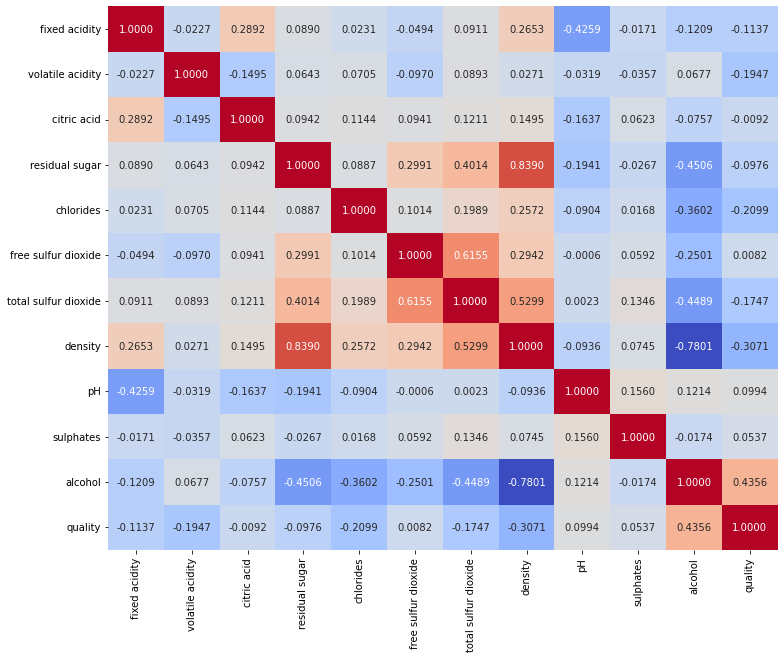
\includegraphics[width=\linewidth]{images/corr.png}
		\caption{Wine Data를 구성하는 각 Column의 Pearson 상관관계를 분석한 그림.}
		\label{fig:corr}
	\end{figure}

	\begin{table}
		\centering
		\begin{tabular}{l|l|l||l|l|l||l|l|l}
			\hline
			\textbf{Variable} & \textbf{Min} & \textbf{Max} & \textbf{Variable}    & \textbf{Min} & \textbf{Max} & \textbf{Variable} & \textbf{Min} & \textbf{Max} \\ \hline
			fixed acidity     & 3.80         & 14.20        & chlorides            & 0.009        & 0.346        & pH                & 2.72         & 3.82         \\ \hline
			volatile acidity  & 0.08         & 1.10         & free sulfur dioxide  & 2.00         & 289.00       & sulphates         & 0.22         & 1.08         \\ \hline
			citric acid       & 0.00         & 1.66         & total sulfur dioxide & 9.00         & 440.00       & alcohol           & 8.00         & 14.20        \\ \hline
			residual sugar    & 0.60         & 65.80        & density              & 0.98711      & 1.03898      & quality           & 3.00         & 9.00         \\ \hline
		\end{tabular}
		\caption{Wine data를 구성하는 Columns의 min/max 값.}
		\label{tab:minmax}
	\end{table}

	\section{실험 진행}
	
	Pearson 상관관계의 값에 따라 입력 데이터를 생성하여 총 3개의 모델을 실험하였다.
	
	\begin{itemize}
		\item Model 1: 11개의 모든 데이터를 Input으로 받아, 7차원의 One-hot vector를 출력하는 모델.
		\item Model 2: 상관 계수의 절댓값이 0.1 이상인 8개의 데이터를 Input으로 받아, 7차원의 One-hot vector를 출력하는 모델.
		\item Model 3: 상관 계수의 절댓값이 0.2 이상인 3개의 데이터를 Input으로 받아, 7차원의 One-hot vector를 출력하는 모델.
	\end{itemize}

	여기에서 출력하는 One-hot vector가 10차원이 아니고 7차원인 이유는 앞선 분석에서 Quality의 범위가 3$\sim$9 였기 때문이다. 이렇게 각 모델의 Input 크기를 다르게 하고, 모델의 구조는 Figure \ref{fig:model}와 같이 설계하였다. 여기에서 \verb|input_dim|은 모델이 받는 입력 vector의 차원 수를 의미한다.
	
	\begin{figure}[h]
		\centering
		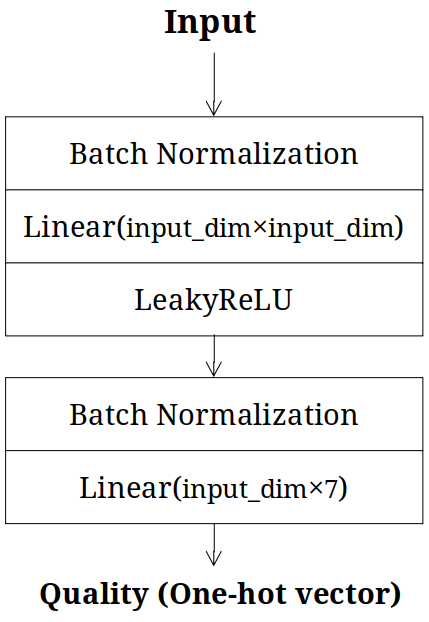
\includegraphics[width=0.3\linewidth]{images/model.png}
		\caption{Quality를 예측하기 위한 모델의 구조.}
		\label{fig:model}
	\end{figure}

	그리고 입력 데이터의 각 변수를 0$\sim$1 사이의 실수 값으로 정규화하는 과정을 거쳤는데, 이는 각 Column에 대하여 최솟값과 최댓값을 구하고 그 값을 이용해 변수의 스케일을 맞추는 것으로 구현되었다. 이후 전체 데이터의 75\% 를 Training 데이터로, 25\% 를 Validation 데이터로 이용하였다.
	
	\begin{table}
		\centering
		\begin{tabular}{l|cc|cc}
			\hline
			\textbf{} & \multicolumn{1}{l}{\textbf{Training Loss}} & \multicolumn{1}{l|}{\textbf{Validation Loss}} & \multicolumn{1}{l}{\textbf{정확히 맞힌 비율}} & \multicolumn{1}{l}{\textbf{1 이하의 차이로 맞힌 비율}} \\ \hline
			Model 1   & \textbf{1.02239}                           & \textbf{1.06640}                              & \textbf{55.61\%}                       & \textbf{95.92\%}                             \\ \hline
			Model 2   & 1.05216                                    & 1.09959                                       & 52.55\%                                & 94.80\%                                      \\ \hline
			Model 3   & 1.16368                                    & 1.14929                                       & 50.41\%                                & 93.57\%                                      \\ \hline
		\end{tabular}
		\caption{각 Model의 Loss와 Validation Data에 대하여 측정된 정확도.}
		\label{tab:results}
	\end{table}
	
	\begin{figure}
		\centering
		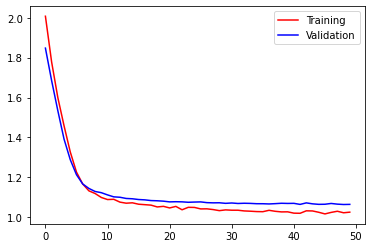
\includegraphics[width=0.3\textwidth]{images/loss1.png}
		\hfill
		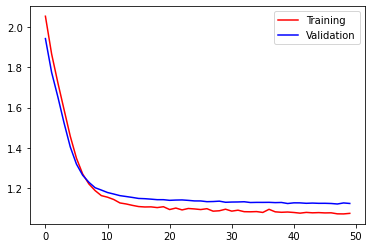
\includegraphics[width=0.3\textwidth]{images/loss2.png}
		\hfill
		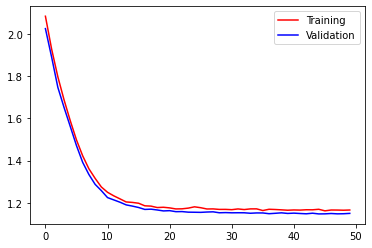
\includegraphics[width=0.3\textwidth]{images/loss3.png}
		\caption{왼쪽부터 오른쪽으로 Model 1, 2, 3를 50 Epochs 동안 학습시킨 결과.}
		\label{fig:results}
	\end{figure}
	
	학습은 50 Epochs 동안 AdamW Optimizer와 MSE Loss를 이용하여 진행되었다. 이렇게 실험한 결과가 Table \ref{tab:results}와 Figure \ref{fig:results}에 정리되어있다. 도출된 결과를 확인하면 상관 계수에 관계없이 모든 변수를 사용한 Model 1이 가장 높은 성능을 보였는데, 이는 모델이 적절한 정규화 기법을 이용한다면 상관관계가 작은 변수라 할 지라도 Overfitting 없이 학습에 도움이 됨을 시사한다.
	
	결과적으로 가장 높은 성능을 보인 Model 1은 Validation 데이터에 대하여 Quality를 정확하게 맞힌 것은 55\% , 1의 오차 범위 내로 맞힌 것은 95\% 로 상당히 준수한 성능을 보였다. 그리고 입력 데이터를 적게 사용한 Model 2, 3는 1보다 나쁜 일반화 성능을 보였다.
	
	
	
\end{document}
